\chapter{Esbeltez de uma viga em relação à resistência característica do concreto}

Diante das vantagens apresentada pelo CUAD como solução construtiva, será feita uma análise comparativa acerca da força de protensão necessária para se aplicar em uma viga, a resistência característica do concreto e a área da seção transversal da viga. O objetivo será analisar a economia de material e o vão que poderá ser vencido. Não serão feitas verificações de estado limite último, estado limite de serviço e fissuração. A viga utilizada neste trabalho se baseia no exemplo publicado por \citeonline[p.~37]{Cholfe}.

\nomenclature[A]{ELU}{Estado limite último}
\nomenclature[A]{ELS}{Estado limite de serviço}

\section{Características}

Neste trabalho, será analisada uma viga de seção T com as características mostradas na \autoref{vigat}.

\begin{figure}[htb]
	\caption{\label{vigat} Detalhes da viga de seção  utilizada no estudo de caso.}
		\begin{center}
			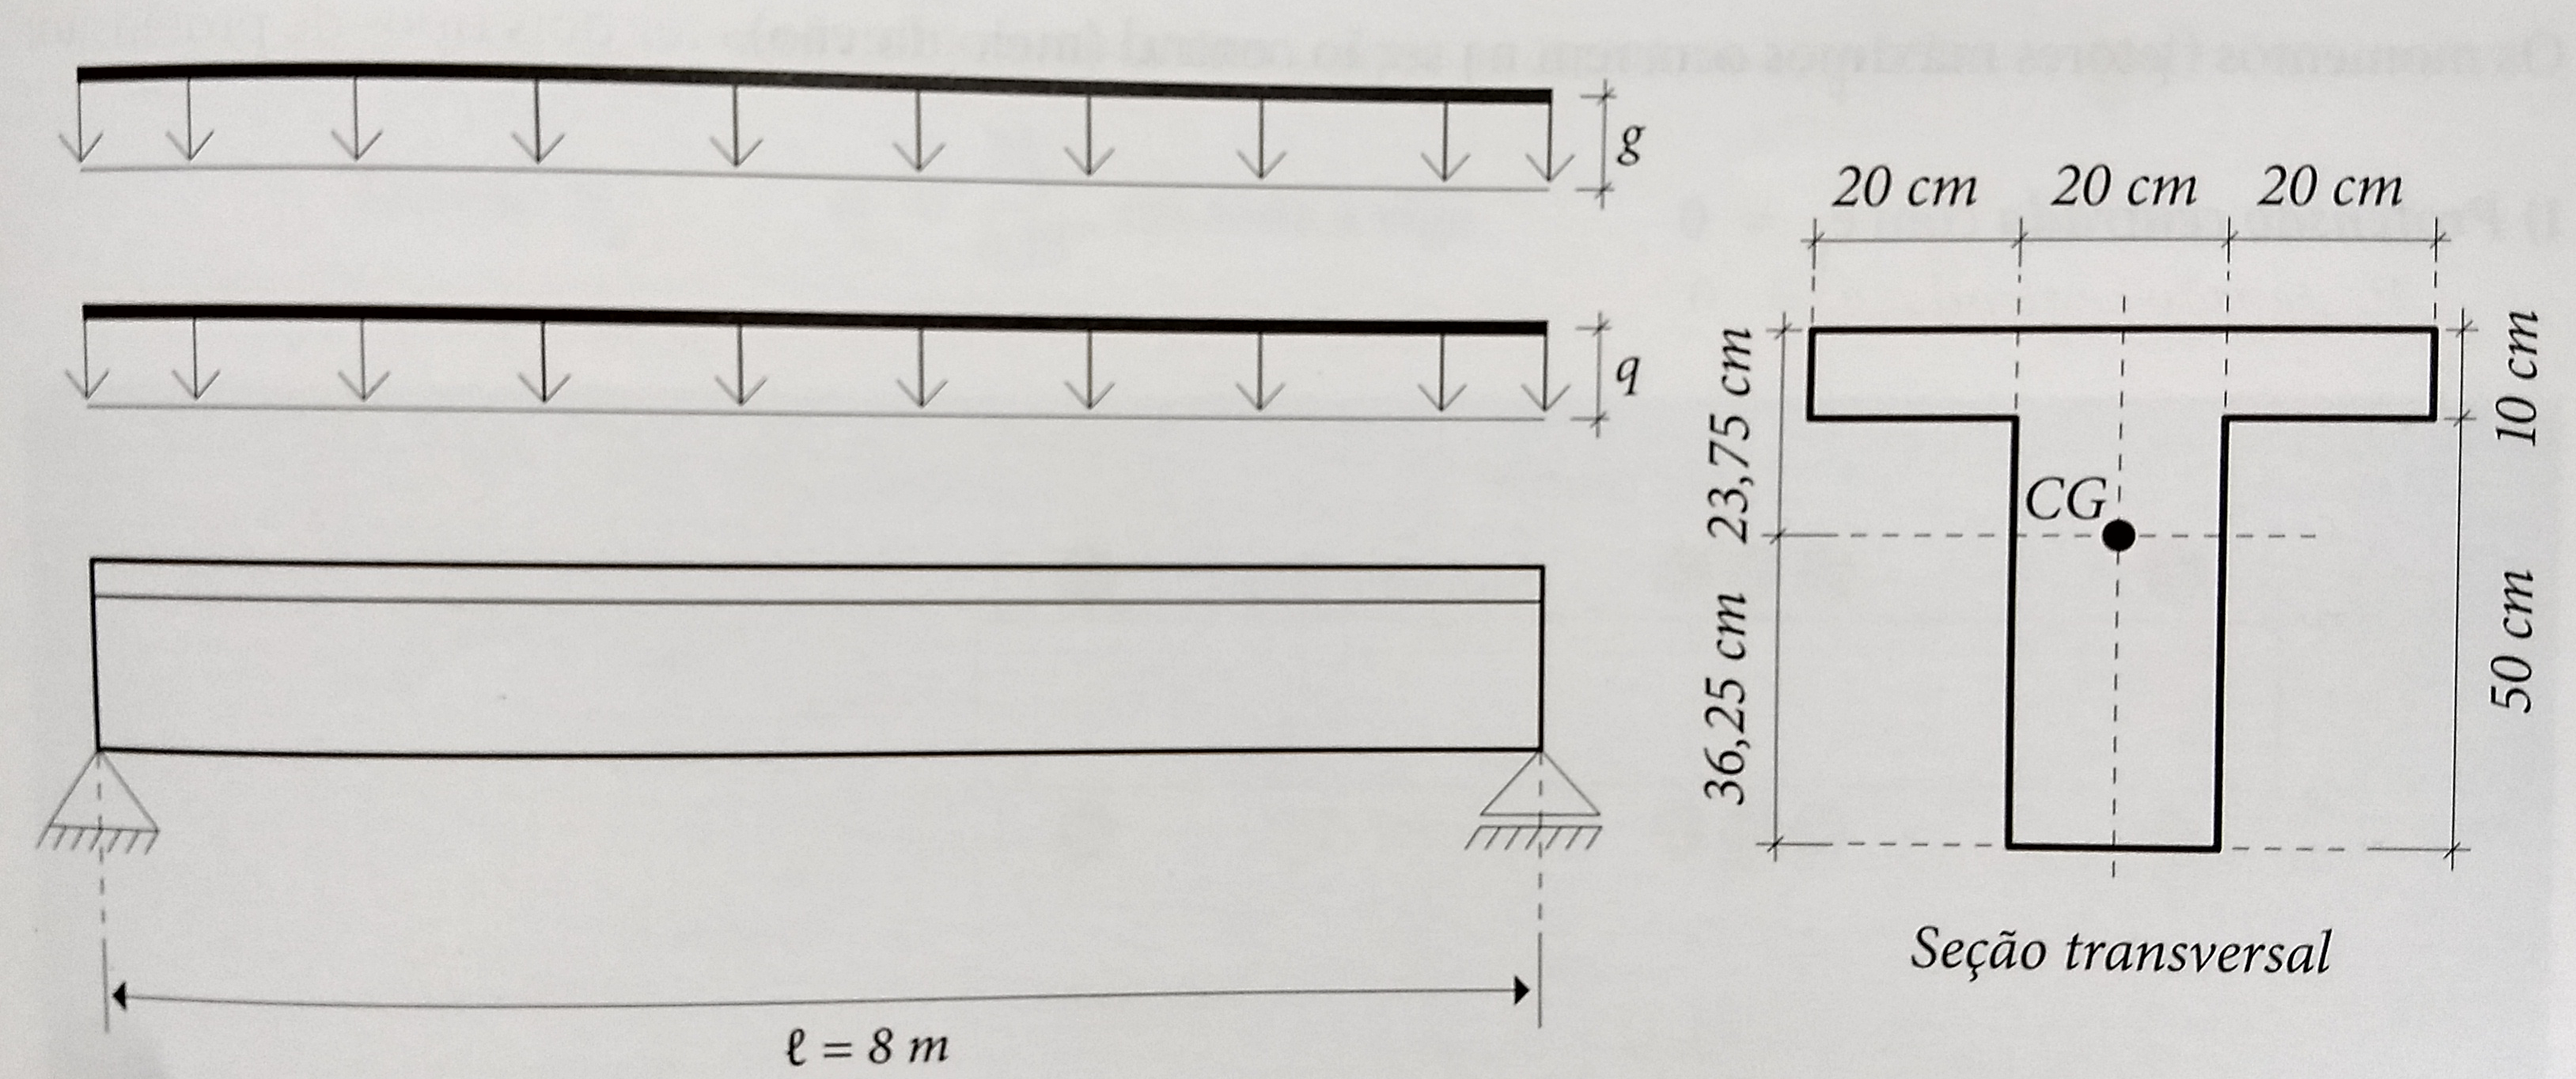
\includegraphics[max width=\textwidth]{viga-t.jpg}
		\end{center}
		\fonte{\citeonline[p.~37]{Cholfe}.}
\end{figure}


O valor da força de protensão será dimensionado considerando o cabo reto e a excentricidade da protensão ($ \text{e}_{\text{p}} $) igual a zero.

\section{Condições de cálculo e aplicação}

O cálculo das características geométricas da seção, esforços solicitantes e tensões normais foram feitas com o programa de código aberto Scilab. O algoritmo utilizado pode ser visto no \autoref{script}. As condições limites utilizadas são:

\begin{alineas}
	\item Não serão permitidas tensões de tração;
	\item Compressão máxima no concreto: $ 0,6 \cdot \text{fck} $.
\end{alineas}

A viga estará submetida às seguintes ações:

\begin{alineas}
	\item Ação permanente (g): 15 kN/m;
	\item Ação variável (q): 12 kN/m.
\end{alineas}

Com os parâmetros de entrada no algoritmo já definidos, foi gerada a \autoref{tabelafck}, onde pode se observar o crescimento do vão teórico que a viga pode vencer ao se aumentar o fck do concreto e a força de protensão aplicada, ainda atendendo as condições limite definidas e sem alterar a sua seção transversal. O  gráfico da \autoref{graficofck} mostra a relação entre o aumento do fck e o vão que uma mesma viga pode vencer.

É importante notar que a rigidez de uma viga feita com CUAD tende a ser maior que a de uma viga feita com concreto convencional, devido ao seu módulo de elasticidade maior: 50 GPa (valor preliminar que pode ser considerado sem testes, conforme as recomendações da AFGC), mas que pode chegar a 70 GPa, por conta das fibras adicionadas, contra um módulo de elasticidade de 56 GPa na condição mais favorável (agregados de basalto e diabásio) para concretos com de até $ \text{fck} = 90 \quad \text{MPa}  $. Ainda assim, uma peça estrutural muito esbelta sobre um vão muito grande pode gerar deformações e fissuras excessivas. As recomendações da \citeonline{AFGC} contém as instruções necessárias para fazer estas verificações no CUAD.

\begin{figure}[htb]
	\caption{\label{graficofck} Relação do aumento do vão teórico (l) a ser vencido em relação ao aumento do fck}
	\begin{center}
		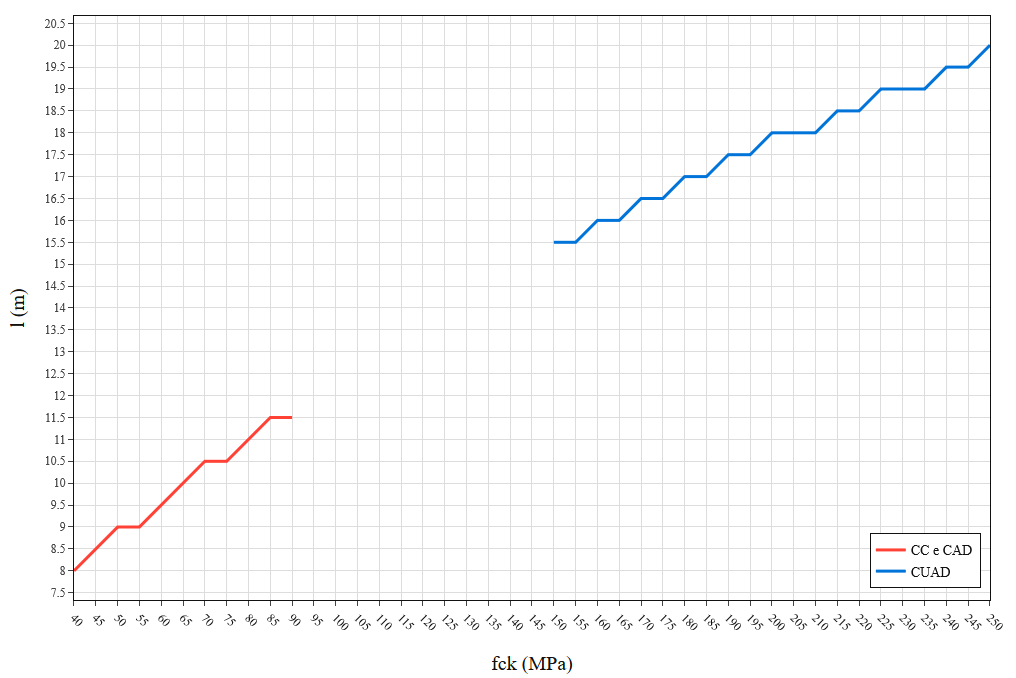
\includegraphics[max width=\textwidth]{Plot4.png}
	\end{center}
%	\fonte{Os autores.}
\end{figure}

%E importante notar que a utilização de seções reduzidas em vigas para vencer grandes vãos pode ser problemática do ponte de vista das deformação da peça. Com $ fck = 40 \text{MPa}$, a rigidez da viga estudada é igual $ kN \cdot m^2 $. Conforme o $ fck $ e o vão teórico aumentam, enquanto a seção transversal

\begin{table}[htb]
	\IBGEtab{%
		\caption{Aumento do fck relacionado ao aumento do vão que a mesma viga pode vencer}
		\label{tabelafck}
	}{%
	\begin{tabulary}{\linewidth}{CCCCC}
		\toprule
		fck do concreto (MPa)	&	Protensão máxima (MPa)	&	Protensão necessária $ \sigma_{c,min} $ (MPa)	&	Aproveitamento da protensão máxima (\%)	&	Vão teórico (m)	\\ \midrule  \midrule
		40,00	&	24,00	&	23,53	&	98,03	&	8,00	\\ \midrule
		45,00	&	27,00	&	26,56	&	98,37	&	8,50	\\ \midrule
		50,00	&	30,00	&	29,78	&	99,26	&	9,00	\\ \midrule
		55,00	&	33,00	&	29,78	&	90,24	&	9,00	\\ \midrule
		60,00	&	36,00	&	33,18	&	92,16	&	9,50	\\ \midrule
		65,00	&	39,00	&	36,76	&	94,26	&	10,00	\\ \midrule
		70,00	&	42,00	&	40,53	&	96,50	&	10,50	\\ \midrule
		75,00	&	45,00	&	40,53	&	90,07	&	10,50	\\ \midrule
		80,00	&	48,00	&	44,48	&	92,67	&	11,00	\\ \midrule
		85,00	&	51,00	&	48,62	&	95,33	&	11,50	\\ \midrule
		90,00	&	54,00	&	48,62	&	90,03	&	11,50	\\ \midrule
		
		150,00	&	90,00	&	88,32	&	98,14	&	15,50	\\ \midrule
		155,00	&	93,00	&	88,32	&	94,97	&	15,50	\\ \midrule
		160,00	&	96,00	&	94,11	&	98,03	&	16,00	\\ \midrule
		165,00	&	99,00	&	94,11	&	95,06	&	16,00	\\ \midrule
		170,00	&	102,00	&	100,09	&	98,12	&	16,50	\\ \midrule
		175,00	&	105,00	&	100,09	&	95,32	&	16,50	\\ \midrule
		180,00	&	108,00	&	106,24	&	98,37	&	17,00	\\ \midrule
		185,00	&	111,00	&	106,24	&	95,71	&	17,00	\\ \midrule
		190,00	&	114,00	&	112,59	&	98,76	&	17,50	\\ \midrule
		195,00	&	117,00	&	112,59	&	96,23	&	17,50	\\ \midrule
		200,00	&	120,00	&	119,11	&	99,26	&	18,00	\\ \midrule
		205,00	&	123,00	&	119,11	&	96,84	&	18,00	\\ \midrule
		210,00	&	126,00	&	119,11	&	94,53	&	18,00	\\ \midrule
		215,00	&	129,00	&	125,82	&	97,53	&	18,50	\\ \midrule
		220,00	&	132,00	&	125,82	&	95,32	&	18,50	\\ \midrule
		225,00	&	135,00	&	132,71	&	98,31	&	19,00	\\ \midrule
		230,00	&	138,00	&	132,71	&	96,17	&	19,00	\\ \midrule
		235,00	&	141,00	&	132,71	&	94,12	&	19,00	\\ \midrule
		240,00	&	144,00	&	139,79	&	97,08	&	19,50	\\ \midrule
		245,00	&	147,00	&	139,79	&	95,09	&	19,50	\\ \midrule
		250,00	&	150,00	&	147,05	&	98,03	&	20,00	\\
		
		\bottomrule
	\end{tabulary}%
}{%
%\fonte{Os autores.}%
%\nota{Recomenda-se o uso de água de amassamento de baixa temperatura, pré cura térmica de 2 dias e cura térmica de 24 horas a uma temperatura de 80\textsuperscript{\degree} C.}
%\nota[Anotações]{Uma anotação adicional, que pode ser seguida de várias outras.}
}
\end{table}

\newpage

Em seguida, comparou-se o quanto a seção da viga T feita com concreto de fck igual a 40 MPa até 90 MPa precisaria aumentar para vencer o mesmo vão de uma viga com as mesmas caraterísticas feitas com um CUAD de fck igual a 150 MPa. Pode-se observar um considerável aumento na área da seção transversal, em comparação com os 0,16 $ \text{m}^2 $ da viga de CUAD. A partir dos resultados mostrados na \autoref{comparacao-cuad-cad}, é possível concluir que as seções de vigas feitas  em CUAD são, aproximadamente, 50\% menores que as feitas de concreto convencional (CC) e concreto de alto desempenho (CAD).

\nomenclature[A]{CC}{Concreto convencional}

\begin{table}[htb]
	\IBGEtab{%
		\caption{Aumento da área da seção transversal}
		\label{comparacao-cuad-cad}
	}{%
	\begin{tabulary}{\linewidth}{CCCCCCC}
		\toprule
		fck (MPa)	&	Área da seção ($\text{m}^2$)	&	Taxa de aumento (\%)	\\ \midrule  \midrule
		40	&	0,453	&	64,64	\\ \midrule
		45	&	0,453	&	64,64	\\ \midrule
		50	&	0,360	&	55,56	\\ \midrule
		55	&	0,338	&	52,59	\\ \midrule
		60	&	0,338	&	52,59	\\ \midrule
		65	&	0,338	&	52,59	\\ \midrule
		70	&	0,338	&	52,59	\\ \midrule
		75	&	0,315	&	49,21	\\ \midrule
		80	&	0,315	&	49,21	\\ \midrule
		85	&	0,263	&	39,05	\\ \midrule
		90	&	0,263	&	39,05	\\ \midrule \midrule
			& \textbf{Média} &	51,91	\\
		\bottomrule
	\end{tabulary}%
}{%
%\fonte{Os autores.}%
%\nota{Recomenda-se o uso de água de amassamento de baixa temperatura, pré cura térmica de 2 dias e cura térmica de 24 horas a uma temperatura de 80\textsuperscript{\degree} C.}
%\nota[Anotações]{Uma anotação adicional, que pode ser seguida de várias outras.}
}
\end{table}



%A partir da análise do gráfico, com o auxílio do Excel, propõe-se a equação \autoref{escolha}, para se ter uma ferramenta fácil para escolher o $ fck $ do concreto para uma viga protendida em relação ao vão teórico a ser vencido.
%
%\begin{equation}
%fck = 0,25 \cdot l^2 + 0,4 \cdot l + 21
%\end{equation}
%
%Onde: 
%
%\begin{alineas}[label=\textbullet]
%	\item $ fck $ = resistência característica do concreto aos 28 dias de idade;
%	\item $ l $ = vão teórico a ser vencido.
%\end{alineas}
